\chapter{Design}
To design and eventually implement a redaction method that strikes a middle ground in terms of safety and accessibility, it's crucial to understand the relevant parts of the internal structure of PDFs. This knowledge allows for direct manipulation, paving the way for an effective redaction method. This chapter provides an overview of important aspects of PDFs and how they can be manipulated to achieve redaction that aligns with this middle ground.

\section{Portable Document Format}
The Portable Document Format (PDF) is designed to present documents, including text formatting and images, independently of application software, hardware, and operating systems.
\subsection{Structure}
A PDF document can be split into 4 distinct parts: 
\\\\
\textbf{Header}. The header of a PDF document serves as its starting point. It contains the critical information about the file which is essential for identifying the PDF format and ensuring compatibility with PDF readers. \\
\textbf{Body}. The body of the PDF contains a series of objects, each represented by a unique object number. These objects can include text, images, fonts, annotations, and more.\\
\textbf{Trailer}. The trailer section provides essential information about the PDF, including the location of the cross-reference table, the size of the file, and other metadata. \\
\textbf{Cross-Reference Table(Xref)}. The cross-reference table provides a map of the location of each object within the PDF file. It helps in quickly locating and accessing specific objects, contributing to the efficiency of document retrieval.
\\\\
The actual contents of a page are often embedded in a stream which is contained in an object, which may contain information about fonts, page content, or acts a reference point to other objects.  
\begin{figure}[h]
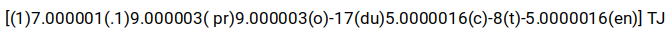
\includegraphics[width=0.85\textwidth]{latex/media/TJexample.png}
\centering
\caption{The TJ text showing operator specifies the glyphs to render (i.e.\textit{( pr)} and \textit{(en)}), along with their widths and associated positional adjustments (i.e.\textit{(9.000003)} and \textit{(-5.0000016)} by the reference to a font object (not shown here). Adjustments are given in text space units. }
\label{fig:tjexample}
\end{figure}
\subsection{Text rendering}
PDF documents can render text in many ways, including by the use of a text showing operator, one of which (TJ) is depicted in figure \ref{fig:tjexample}. The TJ operator takes as arguments a string of text and a vector of positional adjustments which displace the character with respect to its default position. This position is often determined by the previous character on the line, consisting of a fixed offset equivalent to the \textit{advance width} of the previous character, defined elsewhere in the PDF. The string of text may be divided in multiple separate parts, each surrounded by parentheses. In this example, the string '\textit{1.1 producten}' is divided into 8 parts. Each substring may have positional information associated, placed either before or after its position in the operand. 
\\\\
The positional information associated with text poses a security concern. The precise width of a redaction and any positional adjustments of non-redacted text on the same line, conditioned on the positional information of both redacted and non-redacted text before redaction, can be exploited to eliminate potential redacted texts \cite{bland2022story}. The presence or absence of these positonal adjustments depends on the \textit{workflow} that has been used; PDF documents produced by a originating software (referred to as the PDF producer by the ISO 32000 PDF standard) and subsequent software that may have modified the PDF file contents thereafter. When saving an email or using the 'Save as PDF' functionality in Microsoft Word for example, the documents have \textit{dependent} shifting schemes (positional adjustments are dependent on previous words on the same line). In contrast, other workflows may produce documents with \textit{unadjusted}(i.e. independent) shifting schemes, where positional adjustments are not dependent on previous words on the same line
\subsection{Metadata}
A PDF document may contain extra information which is embedded within the PDF document but hidden for the eye \cite{muller2021processing}. This hidden information might include information about the actual textual contents of the document. An example of such hidden information is annotations by authors or reviewers, commenting on specific parts of the document, referring or quoting text which has been redacted from the page, but not from the document. 
\begin{figure}[h]
    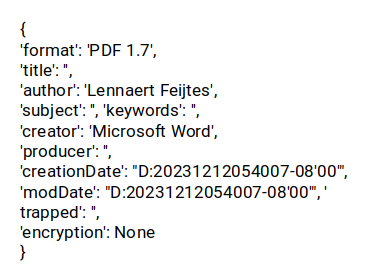
\includegraphics[width=0.5\linewidth]{latex/media/metadata.png}
    \centering
    \caption{An example of metadata which may be present in a PDF document. Information such as the author name, subject and description of the document can be retrieved from the document if not removed.}
    \label{fig:metadataexmp}
\end{figure}\\
Hidden information can take various forms, including standard metadata in the PDF depicted in figure \ref{fig:metadataexmp} or XML-metadata. Additionally, it may be found in file attachments, embedded files, bookmarks, embedded search indices, comments and markups, form fields, transparent text, covered content, hidden layers, deleted or cropped content, or links.
\section{Effective redaction}

Effective redaction involves the removal of information from a PDF document, striking a balance between safeguarding the confidentiality of redacted information and maintaining document accessibility. To achieve this, an effective redaction method would accept as input a PDF document from any source which has been created by any means (workflow), and a list of one or more character sequences along with their bounding boxes per page for redaction. Each of these bounding boxes define areas in the document where content must be removed after redaction.
\\\\
As a result, the redaction method outputs an edited PDF where the specified character sequences have been removed. Both the visual textual content and hidden content have to be checked for the presence of the to-be-removed character sequences. The resulting file should be manipulated to the point where sufficient security has been achieved while the visual style and accessibility of the original document has been maintained as much as possible. 
\\\\
The following criteria must be met in the resulting file:
\begin{enumerate}
    \item The to-be-redacted text has been removed from the visible textual content of the PDF document.
    \item To-be-redacted text is removed from any part of the PDF document, including attached files, metadata, and the table of contents.
    \item Text that should not be removed is retained in visible areas of the file. For non-visible parts (e.g., metadata or file attachments), the option to either remove them entirely or examine and selectively remove to-be-redacted text. 
    \item Text that should not be removed is not altered to the extent that it becomes unreadable by both humans and machines. While changes may occur for security or accessibility reasons, the text should remain readable after manipulation. 
    \item Edited, inserted, repositioned or any other text that has not been deleted may be horizontally moved to the point that it still resembles the layout of the original file. Vertical repositioning must be kept limited to not overlap text on one line with text on another, and other forms of positional adjustments must be kept to a minimum but are allowed as long as they do not result in a too great of a change compared to the original file.
\end{enumerate}
Effective redaction involves several steps:

\begin{enumerate}
    \item \textbf{Labelling text} to distinguish text that should be removed from text that should not be removed. This is achieved by either selecting one or more character sequences throughout the entire file or separately for each page. Different means of labelling may be possible, either though a GUI or manually using a command-line or a separate file. Labelling results in bounding boxes used for locating text.
    
    \item \textbf{Locating text} to be removed by scanning all objects in the PDF document for streams where text is rendered with a sequence of text showing operators. In these streams, both the actual textual contents and their position on a page should be retrieved by retrieving their text showing and positional operator(s) in order to match the to-be-redacted character sequences (bounding boxes) and their representation in the document. 
    
    \item \textbf{Removing text} by manipulating the arguments of text showing operations associated with the to-be-redacted values. These may have to be manipulated only partially or removed in their entirety to redact the actual value from the textual content of the file. Furthermore, operators that define the position of text on a page may have to be removed as well based on the way text is rendered.
    
    \item \textbf{(Optional) insertion of a replacement value} to indicate that text has been redacted from the document. The replacement value could be a fixed value (i.e. REDACTED or [x]) or a value that preserves the semantic meaning of the redacted text and context based on the original value (inspired by \cite{olstad2023generation}). 
    
    \item \label{posadj} \textbf{Manipulation of positional adjustments} that remains after removal of text in order to defend against deredaction. Taking figure \ref{fig:tjexample} as an example, only removing the text within the parentheses is not safe because the positional adjustments associated of the whole text are not manipulated. For every or most characters, changing the positional information or removing it completely increases confidentiality. Following the recommendations of Maxwell Bland (one of the authors of Story Beyond the Eye \cite{bland2022story}, three methods from safer to safest can be derived:
        \begin{enumerate}
            \item \textbf{Make it computationally harder} to guess the redacted text by adding adjustments to every or most characters. This increases the confidentiality of the redacted text while maintaining the same general visual/aesthetic guarantees. 
            \item \label{b} \textbf{Make the adversary guess from more options} rather than one. Mixing in the positional adjustments that would result from 10 other names randomly selected from a given dictionary would increase the number of potential redacted, and would thus make it harder to guess the real redacted value. This approach enhances confidentiality even more while preserving the same general visual layout.
            \item \label{c} \textbf{Removing shifts} entirely from the file. Tools such as Edact-Ray protect vulnerable PDF redactions by providing a configurable level of information excisement to the user, allowing users to optionally remove all non-redacted glyph shifts. Spaces between words are rounded up based on the width of a single character in the monospace font. While these changes guarantee the redactions’ security, it radically changes the document for the eye, which may not be suitable when preserving the layout of the document is crucial.
        \end{enumerate}

        Option \ref{b} and \ref{c} would both require knowledge about the scheme used to determine where positional adjustments should be placed. Reconstructing such a scheme might be a complex and time-consuming task. 
    \item \textbf{(Optional) white space removal} by manipulating text positions of non-redacted words. Words on the same line where text has been removed should be selected for repositioning. For each of these selected words, the position should be manipulated based the redacted value(s), possible replacements values and non-redacted text.
    \item \textbf{Hidden information removal} from the document by first searching for the labelled character sequences. Subsequently, delete them in one or more of the following: (xml) metadata, attachments, bookmarks, embedded search index, comments and markups, form fields, transparent text, covered content, hidden layers, deleted or cropped content or links. An alternative option is to delete one or more of these parts in their entirety from the document; such as the embedded files, comments, attachments and covered/deleted/cropped content. Other parts, such as the table of contents, links and metadata may have to be examined carefully because they also influence non-hidden information to a greater extent. 

\end{enumerate}

